% XeLaTeX

\documentclass[a4paper]{article}
\usepackage{ctex}
\usepackage{xypic}
\usepackage{amsfonts,amssymb}
\usepackage{multirow}
\usepackage{geometry}
\usepackage{graphicx}
\usepackage{listings}
\usepackage{lipsum}
\usepackage{courier}
\usepackage{fancyvrb}
\usepackage{etoolbox}


\linespread{1.2}
\geometry{left=3cm,right=2.5cm,top=2.5cm,bottom=2.5cm}

\makeatletter
\patchcmd{\FV@SetupFont}
  {\FV@BaseLineStretch}
  {\fontencoding{T1}\FV@BaseLineStretch}
  {}{}
\makeatother

\lstset{basicstyle=\small\fontencoding{T1}\ttfamily,breaklines=true}
\lstset{numbers=left,frame=shadowbox,tabsize=4}
%\lstset{extendedchars=false}
\begin{document}

\title{实验八 \ 进程同步机制 \ 实验报告}
\author {数据科学与计算机学院 \ 计算机科学与技术 2016 级 \\ 王凯祺 \ 16337233}
\maketitle

\section{实验目的}

\begin{itemize}
\item 用于互斥和同步的计数信号量机制
\item 多个进程能够利用计数信号量机制实现临界区互斥
\item 合作进程在并发时,利用计数信号量,可以按规定的时序执行各自的操作,实现复杂的同步,确保进程并发的情况正确完成使命
\end{itemize}

\section{实验要求}

\begin{itemize}
\item 内核实现do\_p()原语,在c语言中用p(int sem\_id)调用 
\item 内核实现do\_v()原语,在c语言中用v(int sem\_id)调用
\item 内核实现do\_getsem()原语,在c语言中用getsem(int init\_val)调用,参数为信号量的初值
\item 内核实现do\_freesem(int sem\_id),在c语言中用freesem(int sem\_id)调用
\end{itemize}

\section{实验步骤}

\subsection{解决历史遗留问题}

老师提供的银行存款程序是长这样的:

\begin{lstlisting}[language=C]
include "process.h"
include "sync.h"
int bankbalance=1000;/*银行帐户余额1000元*/
void main() {
	int pid,sem_id;
	int t,totalsave=0,totaldraw=0;
	sem_id=GetSem(1);
	pid=fork();
	if (pid==-1) {printf(“error in fork!”);exit(-1);}
	if (pid)  {
		while (1) {
			p(sem_id);
			t=bankbalance;   /*父进程反复存钱,每次10元*/
			delay(3);
			t=t+10;
			delay(2)
			bankbalance=t; 
			totalsave+=t;
			printf(“bankbalance=%d,%totalsave=%d”, bankbalance,totalsave );
			v(sem_id);
		}
		exit(0);
	} 
	else {
		/*子进程反复取钱,每次20元*/
		exit(0);
	}
}
\end{lstlisting}

我估算了一下这个程序编译后的大小,发现可能远大于 512 字节。由于我在实验三的时候过于自信地认为用户程序应该不会超过 512 字节,所以在内存里为每个用户程序都只预留了 512 字节的空间。在上个实验中, fork 测试程序已经差不多占满了,因此在这个实验中必须得为用户程序扩容。那么,我们需要重新布局软盘空间、重新分配内存空间、修改复制函数。

在实验七中我实现的 fork 是复制进程,而不是复制线程。具体为:复制 CS 、 DS 、 ES 、 SS 中的数据复制一份。现在由于要使用共享变量,必须使用线程而非进程。我只需要不再复制 CS 、 DS 、 ES ,只复制 SS 中的数据。

\subsection{Sleep 函数}

老师的程序里使用了 Sleep 函数,是为了显著增加 RC 问题发生的概率。如果不加 Sleep 函数,此 RC 问题可能要花很长时间才能测试出来。

我使用系统调用来实现 Sleep 函数。用户程序调用 Sleep 函数时,启动中断服务程序。中断服务程序先做 save 操作,然后将当前进程阻塞,并记录该进程还需等待的秒数。每当时钟中断发生时,等待秒数 -1 。当秒数减至 0 时,将当前进程恢复为就绪。

Sleep 中断核心代码展示:

\begin{lstlisting}[language=C]
void sleepint() {
	int sleeptime;
	save();
	sleeptime = new_pcb.ax;
	if (sleeptime > 0) {
		PCBlist[now_process].status = BLOCK;
		sleepqueue[sleepqueue_top].val = now_process;
		sleepqueue[sleepqueue_top].sleeptime = sleeptime;
		++ sleepqueue_top;
	}
	exchange();
}
\end{lstlisting}

时钟中断核心代码展示:

\begin{lstlisting}[language=C]
void timeint() {
	int i, j;
	save();
	for (i = 0; i < sleepqueue_top; ++i) {
		sleepqueue[i].sleeptime -= 1;
		if (sleepqueue[i].sleeptime <= 0) {
			PCBlist[sleepqueue[i].val].status = READY;
			for (j = i; j + 1 < sleepqueue_top; ++j) {
				sleepqueue[j].val = sleepqueue[j + 1].val;
				sleepqueue[j].sleeptime = sleepqueue[j + 1].sleeptime;
			}
			-- i;
			-- sleepqueue_top;
		}
	}
	exchange();
}
\end{lstlisting}

\subsection{测试 RC 问题}

我将老师的代码有关信号量的函数全部删去,测试一下是否真的会产生 RC 问题。

测试代码如下:

\begin{lstlisting}[language=C]
#include "stdlib.h"
#include "stdio.h"
#include "sync.h"

int bankbalance = 1000;

void syncmain() {
	int pid, sem_id;
	int t, i;
/*	sem_id = getSem(1);  */
	if (sem_id >= 0 && sem_id < 64) {
		puts_no_new_line("Applying signal: sem_id = ");
		printint(sem_id);
	} else {
		puts("error while applying signal");
	}
	pid = fork();
	if (pid == -1) {
		puts("error in fork!");
		exit(-1);
	}
	if (pid) {
		puts("father process: fork OK");
		sleep(2);
		puts("father process: sleep OK");
		while (1) {
/*			P(sem_id);  */
			t = bankbalance;
			sleep(3);
			t = t + 10;
			sleep(2);
			bankbalance = t;
			puts_no_new_line("+10, bankbalance = ");
			printint(bankbalance);
/*			V(sem_id);  */
		}
		exit(0);
	} else {
		puts("child process: fork OK");
		sleep(2);
		puts("child process: sleep OK");
		while (1) {
/*			P(sem_id);  */
			t = bankbalance;
			sleep(3);
			t = t - 20;
			sleep(2);
			if (t >= 0) {
				bankbalance = t;
				puts_no_new_line("-20, bankbalance = ");
				printint(bankbalance);
			} else {
				puts("money not enough!");
			}
/*			V(sem_id);  */
		}
		exit(0);
	}
}
\end{lstlisting}

运行结果如下:

\begin{figure}[!hbp]
	\centering
	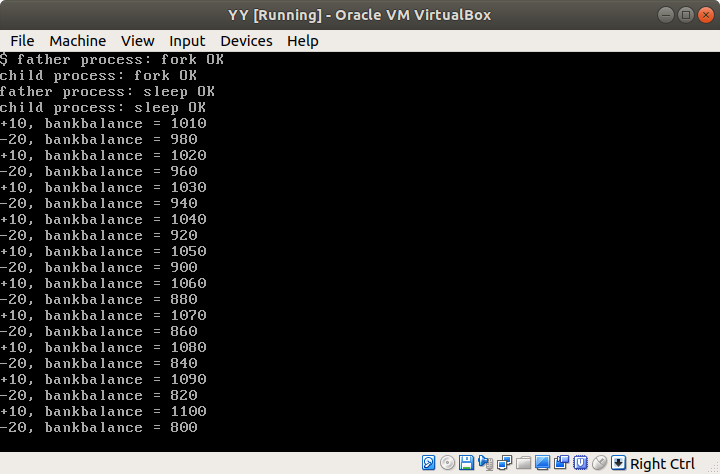
\includegraphics[scale=0.55]{pics/1.png}
\end{figure}

RC 问题在第一次取款的时候就出现了!如果只有这一张截图,并不能证明就是 RC 问题的锅。 RC 问题的根源是两个进程共享变量,如果这个变量是私有的,那么上面这张截图是正常的。

\newpage

\begin{figure}[!hbp]
	\centering
	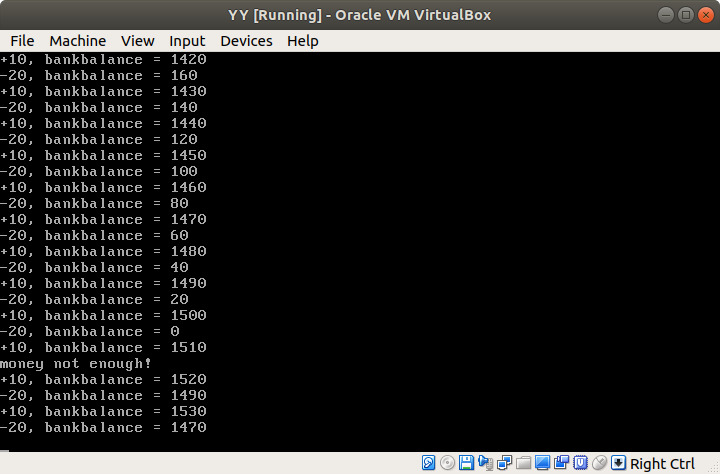
\includegraphics[scale=0.55]{pics/2.png}
\end{figure}

我们耐心地等 bankbalance 跑到 0 ,在不够钱的下一次取款,余额重新回到 1490 ,证明了 bankbalance 这个变量是共享变量。导致账面出错的原因就是 RC 问题。

\subsection{设计信号量数组}

\begin{lstlisting}[language=C]
int signalav[64];        // 表示信号量是否被使用
int signal[64];          // 表示信号量的值
int signalqueue_top[64]; // 表示信号量队列长度
int signalqueue[64][64]; // 表示信号量队列(进程编号)
\end{lstlisting}

本来想用指针实现队列的,我不会写动态内存分配还是算了吧……

\subsection{设计信号量中断服务程序}

我给信号量中断服务程序分配了一个中断号: 25h ,再对 4 个功能分别分配功能号。

\begin{table}[!hbp]
\centering
\begin{tabular}{|l|l|l|l|l|}
\hline
函数 & 功能 & 功能号 & 传入参数 & 返回参数 \\
\hline
getSem & 申请一个新的信号量 & ah = 00h & dx = 初值 & ax = 信号量编号 \\
\hline
P & P 操作 & ah = 01h & dx = 信号量编号 & - \\
\hline
V & V 操作 & ah = 02h & dx = 信号量编号 & - \\
\hline
freeSem & 释放一个信号量 & ah = 03h & dx = 信号量编号 & - \\
\hline
\end{tabular}
\end{table}

核心代码如下:

\begin{lstlisting}[language=C]
void signalint() {
	int p, d, i, ok;
	save();
	p = new_pcb.ax >> 8;
	d = new_pcb.dx;
	if (p == 0x0) {
		ok = -1;
		if (d > 0) {
			for (i = 0; i < 64; ++i)
				if (signalav[i] == 0) {
					signalav[i] = 1;
					signal[i] = d;
					ok = i;
					break;
				}
		}
		new_pcb.ax = ok;
	} else
	if (p == 0x1) {
		if (d >= 0 && d < 64 && signalav[d]) {
			-- signal[d];
			if (signal[d] < 0) {
				signalqueue[d][ signalqueue_top[d]++ ] = now_process;
				PCBlist[now_process].status = BLOCK;
			}
		}
	} else
	if (p == 0x2) {
		if (d >= 0 && d < 64 && signalav[d]) {
			++ signal[d];
			if (signal[d] <= 0) {
				PCBlist[ signalqueue[d][0] ].status = READY;
				for (i = 0; i + 1 < signalqueue_top[d]; ++i)
					signalqueue[d][i] = signalqueue[d][i + 1];
				-- signalqueue_top[d];
			}
		}
	} else
	if (p == 0x3) {
		if (d >= 0 && d < 64 && signalav[d]) {
			signalav[d] = 0;
		}
	}
	exchange();
}
\end{lstlisting}

\subsection{再次测试 RC 问题}

做好信号量的工作后,将之前的测试代码加上信号量进行测试。

\newpage

\begin{figure}[!hbp]
	\centering
	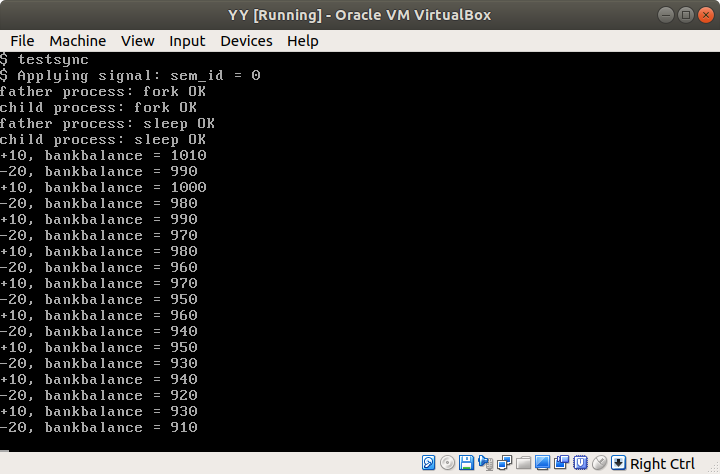
\includegraphics[scale=0.55]{pics/3.png}
\end{figure}

在上图中我们可以看到 RC 问题已经得到解决。账平了!

\begin{figure}[!hbp]
	\centering
	
\includegraphics[scale=0.55]{pics/4.png}
\end{figure}

再上一张图,是儿子取完钱没钱了,RC 问题也没出问题。

\section{实验总结}

单纯信号量这个实验来说,在充分理解信号量原理的基础上实现,还是挺简单的。我花了 1 个小时写好调好 Sleep 函数,再花 1 个小时写好调好信号量。最花时间的是解决历史遗留问题。特别是之前对未来的预判不足,导致资源不足,需要花大量的精力来扩展资源。同样的事情也发生在 Youtube ,Youtube 没有预料到有视频的点赞数会超过 32 位整型的范围,故点赞数量是用 32 位整型存储的。结果那一夜,小苹果的视频点赞量爆 int 了……更新整个数据库是个非常庞大的工程。如果在之前有预见,做好扩展的准备,就不会这么麻烦。

同样的事情也应用在 FAT32 文件系统上,也是由于使用了 32 位整型,单文件大小最大为 4GB 。随着科技的发展, 4GB 的单文件大小明显不够用,那么又要写一套新的文件系统。我觉得程序的可扩展性是非常重要的,无论在何时,都不要想着用户资源“应该”不会超过多少 GB ,而要随时保留扩展的余地(当然,我现在从原来假定用户程序不超过 512 字节改成假定用户程序不超过 4KB ,也没有保留未来扩展的余地,要是程序超过 4KB ,我又要去改内核了)。


\end{document}
















